%%%%%%%%%%%%%%%%%%%%%%%%%%%%%%%%%%%%%%%%%%%%%%%%%%%%%%%%%%%%%%%%%%%%%%%%%%%%%%%%

% preamble

\documentclass[twocolumn]{cinc}
\usepackage{mathtools, graphicx, xurl, hyperref}
% \usepackage{tikz-cd}
\usepackage{tikz}
\usetikzlibrary{shapes,arrows,external,decorations.pathmorphing,backgrounds,positioning,fit,petri,calc,hobby,cd}
% \tikzexternalize[prefix=tikz/,optimize command away=\includepdf]
\usepackage{boldline,multirow}
\usepackage{booktabs} % Allows the use of \toprule, \midrule and \bottomrule in tables
\usepackage{subcaption}
\usepackage{relsize}
\usepackage[ruled,vlined]{algorithm2e}

% \tikzstyle{smallcircleblock} = [circle, draw, text width = 0.7em, text centered]

% \tikzstyle{wideblock} = [rectangle, draw, text width = 6.5em, text centered, rounded corners, inner sep = 7pt, minimum height = 1.0em]


%%%%%%%%%%%%%%%%%%%%%%%%%%%%%%%%%%%%%%%%%%%%%%%%%%%%%%%%%%%%%%%%%%%%%%%%%%%%%%%%

% title, author, institution

\title{Searching for Effective Neural Network Architectures for Heart Murmur Detection from Phonocardiogram}
\author{Hao Wen\textsuperscript{1},
Jingsu Kang\textsuperscript{2} \\ \ \\
\textsuperscript{1}LMIB and School of Mathematical Sciences, Beihang University, Beijing, China\\
\textsuperscript{2}Tianjin Medical University, Tianjin, China
}

\begin{document}
\maketitle


%%%%%%%%%%%%%%%%%%%%%%%%%%%%%%%%%%%%%%%%%%%%%%%%%%%%%%%%%%%%%%%%%%%%%%%%%%%%%%%%

% abstract

\begin{abstract}

% finished

Aim: This work studies the problem of predicting neurological recovery from coma with longitudinal electroencephalogram (EEG) recordings raised by the George B. Moody PhysioNet Challenge 2023.

Methods: Deep neural network (DNN) models were trained to predict cerebral performance category (CPC) scale (1 to 5) from bipolar EEGs which were rescaled to zero mean and unit variance. The prediction was treated as a 5-class classification task. The models adopted a bottleneck SE-ResNet backbone with long short-term memory (LSTM) and global attention modules on its top.

Via a stratified splitting, 20\% of the training data were left out as a validation set for model selection. Recordings were chosen and sliced according to the pre-computed signal quality index for training. The AdamW optimizer and the OneCycle scheduler were used to optimize model weights on the asymmetric loss of the training data. Predictions of multiple EEG recordings from one patient were merged via voting strategies to give a final prediction.

Results: Our team's (''Revenger'') best submission entry received a challenge score of 0.701 for the clinical outcome prediction on the hidden validation set.
% Scores on the 12h/24h/48h subsets were 0.33, 0.4, 0.75 respectively.

Conclusion: Our solution offers a practical way to continuously monitor the brain after cardiac arrest using EEGs, with room and potential for further enhancements.

\end{abstract}


% main body of the paper

\section{Introduction}
\label{sec:intro}

% almost finished

Cardiac arrest (CA), especially out-of-hospital cardiac arrest (OHCA), is a major worldwide public health issue with a low survival rate \cite{Yan_2020_Global}. CA often results in cerebral lesions, a leading cause of early death for patients resuscitated from it \cite{Benghanem_2022_Prog}. Physicians prognosticate the neurological recovery outcomes for survivors comatose after initial treatments \cite{Cronberg_2020_Brain}, which is a challenging task requiring a minimal false-positive rate of poor outcomes.

With the aim of improving objectivity and accessibility for reliable prognostication after CA, the George B. Moody PhysioNet Challenge 2023 \cite{Goldberger2000, 2023Challenge} proposed to develop automated auxiliary prognostic support systems using longitudinal EEG. In this work, a novel approach providing qualitative neurological interpretations and predictions is presented.


\section{Methods}
\label{sec:methods}

% NOT finished

\subsection{Dataset and SQI-based Data Selection}
\label{subsec:data_selection}
% almost finished

The public dataset for the Challenge is the International Cardiac Arrest REsearch consortium (I-CARE) database \cite{Amorim_2023_ICAREDatabase}. It contains mainly EEG recordings from comatose patients with cardiac arrest which were collected up to 72 hours from their return of spontaneous circulation (ROSC). Although this dataset contains physiological signals other than EEG, we base this study only on the EEG data for the following 2 reasons:
\begin{itemize}
    \item The amount of EEG data in the public dataset is already enormous, exceeding 30,000 hours in length.
    \item Previous literature \cite{Zheng_2021_coma} has illustrated the feasibility of using EEG as the sole physiological signal source on the problem this work considers.
\end{itemize}

As the computation resources and execution time are limited under the circumstances of the Challenge, further offline data selection was conducted according to the signal quality index (SQI) of the EEGs. The SQI was computed for every 5-minute epoch as its proportion of ``normal'' 10s segments. A 10s segment is regarded as ``normal'' if no artefact is detected from it, including abnormal values and patterns in the waveform and in the spectrum \footnote{Refer to \url{https://github.com/DeepPSP/cinc2023/blob/master/utils/artifact_pipeline} for more details.}
% The distribution of SQI for all 5-minute epochs is collected in Figure \ref{fig:sqi-stats}.
At most one epoch was chosen (requiring SQI $\ge 0.95$) from each EEG recording as a representative of it for developing our neural network (NN) models (models will be discussed in Section \ref{subsec:models}). The total number of 5-minute epochs selected was 23350.

% \begin{figure}[!htp]
% \centering
% 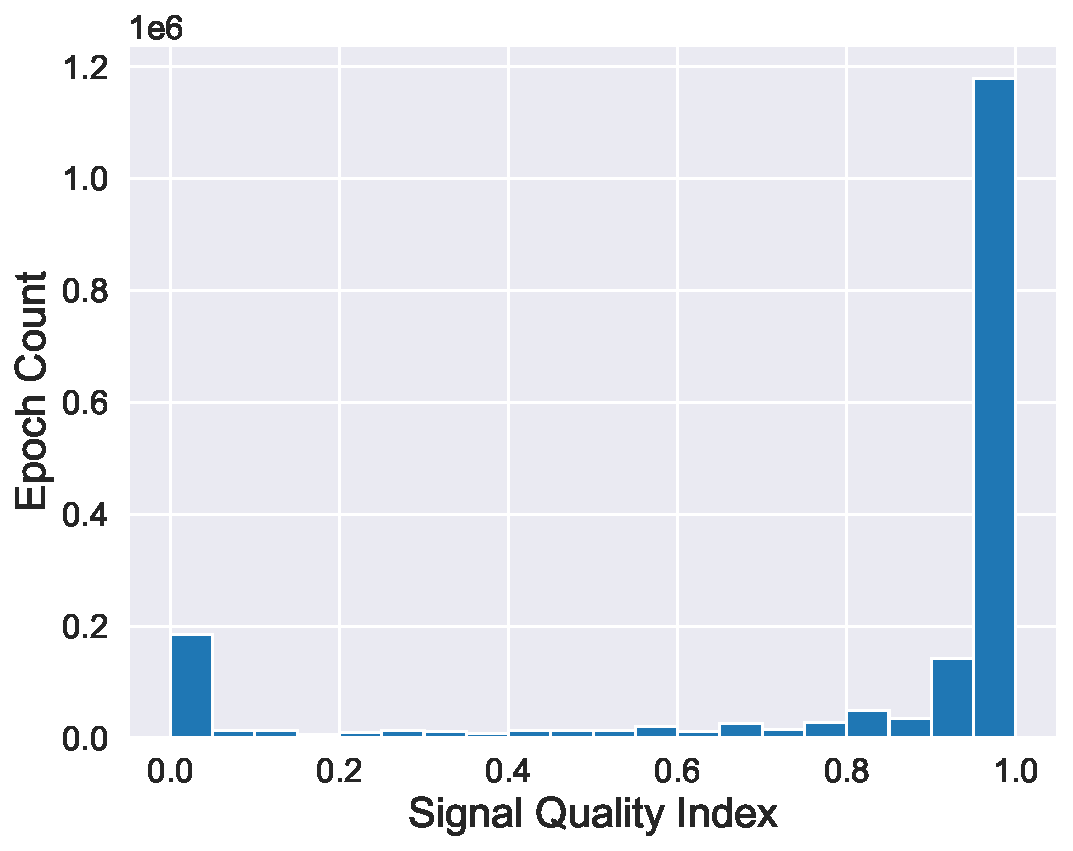
\includegraphics[width=0.95\linewidth]{images/sqi-stats.pdf}
% \caption[]{Distribution of SQI for all 5-minute EEG epochs. Consecutive epochs from one EEG recording have a 1-minute gap (hop length).}
% \label{fig:sqi-stats}
% \end{figure}


\subsection{Preprocessing Criteria}
\label{subsec:data_preproc}
% almost finished

In this subsection, we describe our preprocessing pipeline for model development and making inferences.

The EEG recordings provided by the I-CARE dataset have varying numbers (19 - 21) of channels but share a common set of 19 channels. The voltage values of each EEG signal are relative to an ``unknown'' reference potential. Hence in order to align these voltage values, the varying-dimensional EEG signals were transformed into the bipolar format with the following 18 channels
\begin{indentedquote}{0.3in}
\it Fp1-F7, F7-T3, T3-T5, T5-O1, Fp2-F8, F8-T4, T4-T6, T6-O2, Fp1-F3, F3-C3, C3-P3, P3-O1, Fp2-F4, F4-C4, C4-P4, P4-O2, Fz-Cz, Cz-Pz
\end{indentedquote}
Bipolar values were obtained by subtracting the latter channel from the former channel of the above 18 pairs.
% The number 18 was chosen since it's the smallest number of bipolar channels to reconstruct the original 19-channel EEG signal.

Bipolar EEGs were further standardized with the following 3 sequential operations:
\begin{itemize}
    \item resample to 100 Hz using polyphase filtering;
    \item Butterworth bandpass filter of order 4 and cutoff frequencies 0.5 - 30 Hz;
    \item rescale to zero mean and unit variance (also called z-score normalization).
\end{itemize}

It has to be emphasized that the z-score normalization is a crucial step, without which the model performance degraded significantly as observed in offline experiments which is demonstrated in Figure \ref{fig:train_scores_compare}.

\begin{figure}[!htp]
\centering
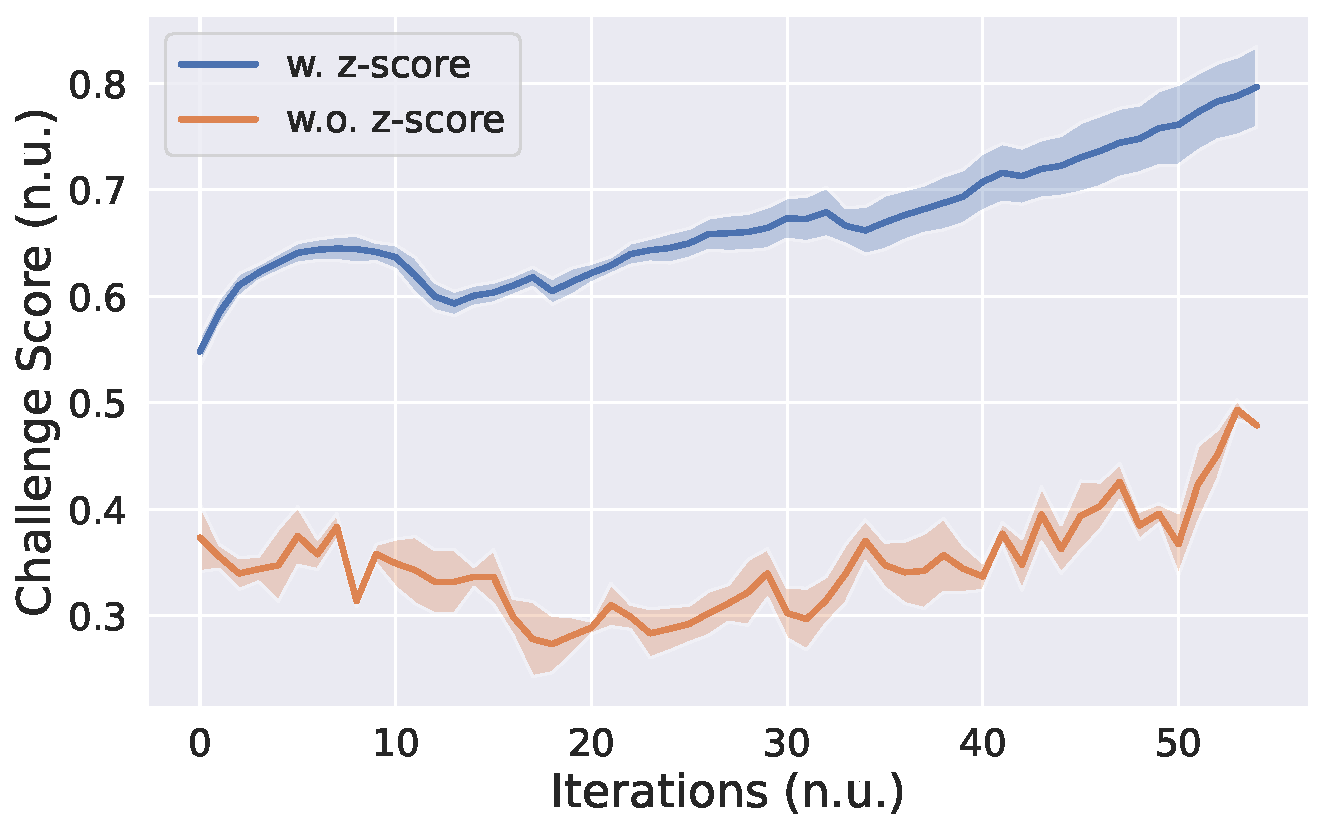
\includegraphics[width=0.95\linewidth]{images/train_scores_compare.pdf}
\caption[]{Comparison between mean curves of challenge scores from multiple experiments on the training set with (w.) and without (w.o.) z-score normalization. Shaded areas are error bounds (standard error of the mean).}
\label{fig:train_scores_compare}
\end{figure}

\subsection{Neural Network Model Selection}
\label{subsec:models}
% almost finished

Considering that there's a clear and widely accepted (also adopted in the Challenge) mapping from CPC scores to clinical outcomes as follows:
\begin{equation}
\label{eq:cpc_outcome_mapping}
\begin{array}{cl}
\text{``Good outcome''} & \text{for CPC score } \in \{1, 2\}; \\
\text{``Poor outcome''} & \text{for CPC score } \in \{3, 4, 5\},
\end{array}
\end{equation}
% \begin{itemize}
%     \item ``Good outcome'' for CPC score $\in \{1, 2\};$
%     \item ``Poor outcome'' for CPC score $\in \{3, 4, 5\},$
% \end{itemize}
and that the CPC scores are discrete scalars, we regard the problem as a 5-class classification problem, i.e. predicting the 5 discrete CPC scores.

A Time-incremental Convolutional Recurrent Neural Network (TiCRNN) \cite{Kang_2022_cinc2021_iop} was adopted as the CPC score classifier. Models with CRNN architecture, especially those with SE-ResNet \cite{hu2020senet} CNN backbones, have proven effective in various physiological signal processing tasks \cite{Kang_2022_cinc2021_iop, wen_cinc2022}. The building block of the SE-ResNet backbone used in this work consists of 3 sequential convolutional blocks of bottleneck shape followed by an SE (squeeze-and-excitation) block with an extra shortcut connecting the input and output as sketched in Figure \ref{fig:se_bottleneck}. The whole architecture of the TiCRNN model used in this work is depicted in Figure \ref{fig:model_arch}. It is a sequential model with 1 stem convolutional block which takes preprocessed EEG waveforms as input, 4 SE-Bottleneck blocks, 2 bidirectional LSTM blocks, 1 SE global attention module, 1 adaptive average pooling layer which outputs the feature vectors, and a multi-layer perceptron which takes in the feature vectors and outputs the probability vectors for the 5 CPC scores.

\begin{figure}[!htp]
\centering
\begin{figure}
\centering

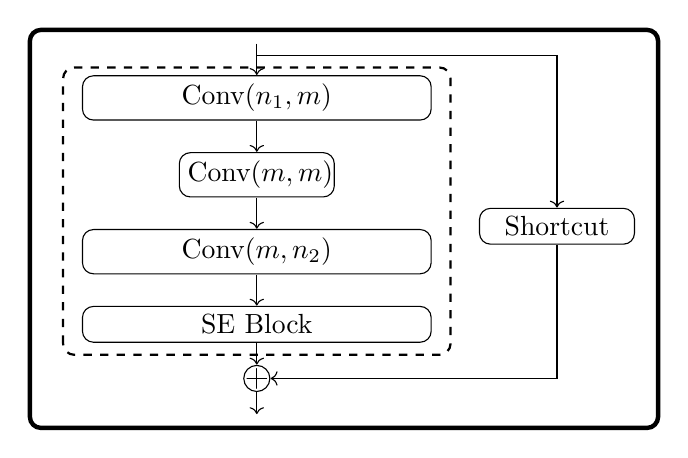
\begin{tikzpicture}%[node distance = 1cm, auto]

\tikzstyle{block} = [rectangle, draw, text width = 5em, text centered, rounded corners, inner sep = 3pt, minimum height = 1.0em]

\tikzstyle{wideblock} = [rectangle, draw, text width = 12em, text centered, rounded corners, inner sep = 3pt, minimum height = 1.0em]

\tikzset{%
  do path picture/.style={%
    path picture={%
      \pgfpointdiff{\pgfpointanchor{path picture bounding box}{south west}}%
        {\pgfpointanchor{path picture bounding box}{north east}}%
      \pgfgetlastxy\x\y%
      \tikzset{x=\x/2,y=\y/2}%
      #1
    }
  },
  plus/.style={do path picture={    
    \draw [line cap=round] (-3/4,0) -- (3/4,0) (0,-3/4) -- (0,3/4);
  }}
}

\coordinate (top) at (0, 0);
\pgfmathsetmacro\blockdist {0.4}
\pgfmathsetmacro\pathshift {0.1}

\node [wideblock, below = \blockdist of top] (conv1) {Conv($n_1, m)$};
\path [->] (top) edge ([yshift = \pathshift]conv1.north);

\node [block, below = \blockdist of conv1] (conv2) {Conv($m, m)$};
\path [->] ([yshift = -\pathshift]conv1.south) edge ([yshift = \pathshift]conv2.north);

\node [wideblock, below = \blockdist of conv2] (conv3) {Conv($m, n_2)$};
\path [->] ([yshift = -\pathshift]conv2.south) edge ([yshift = \pathshift]conv3.north);

\node [wideblock, below = \blockdist of conv3] (se) {SE Block};
\path [->] ([yshift = -\pathshift]conv3.south) edge ([yshift = \pathshift]se.north);

\node [circle, draw, plus, below = 0.7 * \blockdist of se] (plus) {};
\path [->] ([yshift = -\pathshift]se.south) edge ([yshift = \pathshift]plus.north);

\coordinate[below = 0.7 * \blockdist of plus] (bottom);
\path [->] ([yshift = -\pathshift]plus.south) edge (bottom);

\node [block, above right = -0.2 and 0.6 of conv3] (shortcut) {Shortcut};
\draw [->] ([yshift = 7]conv1.north) -| ([yshift = \pathshift]shortcut.north);
\draw [->] ([yshift = -\pathshift]shortcut.south) |- ([xshift = \pathshift]plus.east);


\draw[rounded corners, dashed, thick] ([xshift = -70, yshift = -11]se) rectangle ([xshift = 70, yshift = 11]conv1);
\draw[rounded corners, ultra thick] ([xshift = -82, yshift = -5]bottom) rectangle ([xshift = 145, yshift = 5]top);

\end{tikzpicture}

\caption{The structure of an SE-Bottleneck block. The mainstream in the dashed box consists of 3 convolutional blocks (actually compositions of convolution, batch normalization and activation) followed by an SE block. The channels $n_1, n_2$ are typically several times of $m,$ hence giving the name ``bottleneck''. The shortcut is typically convolutions of kernel size 1, whose stride and input/output channels match the mainstream.}
\label{fig:se_bottleneck}
\end{figure}

\caption{The structure of an SE-Bottleneck block. The mainstream in the dashed box consists of 3 convolutional blocks (actually compositions of convolution, batch normalization and activation) followed by an SE block. The channels $n_1, n_2$ are typically several times of $m,$ hence giving the name ``bottleneck''. The shortcut is typically convolutions of kernel size 1, whose stride and input/output channels match the mainstream.}
\label{fig:se_bottleneck}
\end{figure}

\begin{figure}[!htp]
\centering
% finished

\begin{tikzpicture}%[node distance = 1cm, auto]

% \tikzstyle{block} = [rectangle, draw, text width = 5em, text centered, rounded corners, inner sep = 3pt, minimum height = 1.0em]

\tikzstyle{wideblock} = [rectangle, draw, text width = 12em, text centered, rounded corners, inner sep = 3pt, minimum height = 1.0em]

\pgfmathsetmacro\blockdist {0.4}
\pgfmathsetmacro\pathshift {0.1}

\node [rectangle, text width = 12em, text centered, rounded corners, inner sep = 3pt, minimum height = 1.0em] (input) {EEG Waveform};

\node [wideblock, below = \blockdist of input] (stem) {Stem Conv};
\path[->] ([yshift = -\pathshift]input.south) edge ([yshift = \pathshift]stem.north);

\ifcoloredtext
\node [wideblock, below = \blockdist of stem] (bottleneck) {\bf\color{red}4 $\times$ SE-Bottleneck};
\path[->] ([yshift = -\pathshift]stem.south) edge ([yshift = \pathshift]bottleneck.north);
\else
\node [wideblock, below = \blockdist of stem] (bottleneck) {\bf 4 $\times$ SE-Bottleneck};
\path[->] ([yshift = -\pathshift]stem.south) edge ([yshift = \pathshift]bottleneck.north);
\fi

\node [wideblock, below = \blockdist of bottleneck] (lstm) {2 $\times$ Bidirectional LSTM};
\path[->] ([yshift = -\pathshift]bottleneck.south) edge ([yshift = \pathshift]lstm.north);

\node [wideblock, below = \blockdist of lstm] (se) {SE Global Attention};
\path[->] ([yshift = -\pathshift]lstm.south) edge ([yshift = \pathshift]se.north);

\node [wideblock, below = \blockdist of se] (pool) {Adaptive Average Pooling};
\path[->] ([yshift = -\pathshift]se.south) edge ([yshift = \pathshift]pool.north);

\node [wideblock, below = \blockdist of pool] (mlp) {Multi-Layer Perceptron};
\path[->] ([yshift = -\pathshift]pool.south) edge ([yshift = \pathshift]mlp.north);

\node [rectangle, text width = 12em, text centered, rounded corners, inner sep = 3pt, minimum height = 1.0em, below = \blockdist of mlp] (prob) {Probability Vectors for 5 CPC Scores};
\path[->] ([yshift = -\pathshift]mlp.south) edge ([yshift = \pathshift]prob.north);

\draw[rounded corners, dashed, thick] ([xshift = -80, yshift = -5]mlp.south) rectangle ([xshift = 80, yshift = 5]stem.north);
\ifboxednn
\draw[rounded corners, ultra thick] ([xshift = -103, yshift = -5]prob.south) rectangle ([xshift = 103, yshift = 5]input.north);
\fi

\end{tikzpicture}

\caption{Architecture of the TiCRNN model. Considering that the preprocessed input EEG waveforms have a sampling frequency of 100 Hz, convolutions, except the shortcuts in SE-Bottleneck blocks, have a kernel size of 3. The total number of trainable parameters in 92M.}
\label{fig:model_arch}
\end{figure}

Probability vectors from multiple EEGs of one patient are averaged and re-normalized via softmax to get the final CPC score predictions. The binary clinical outcomes (good, poor) are obtained by applying the mapping \eqref{eq:cpc_outcome_mapping}.

\subsection{Training Strategies}
\label{subsec:training}
% almost finished

As can be inferred from Figure \ref{fig:cpc_vfib_corr}, We have a highly imbalanced distribution of the learning objective (the CPC score) in the I-CARE dataset, which is also divergent across different hospitals as illustrated in Figure \ref{fig:outcome_hospital_corr}. Therefore, the asymmetric loss \cite{ridnik2021asymmetric_loss}, which is the state-of-the-art loss function for multi-label (and also for multi-class) classification problems, was chosen as the minimizing objective. The self-adaptive optimizer \texttt{AdamW} was used in conjunction with the \texttt{OneCycle} scheduler to incrementally update the NN model weights towards their optimal.

\begin{figure}[!htp]
\centering
\begin{subfigure}[t]{0.49\linewidth}
    \centering
    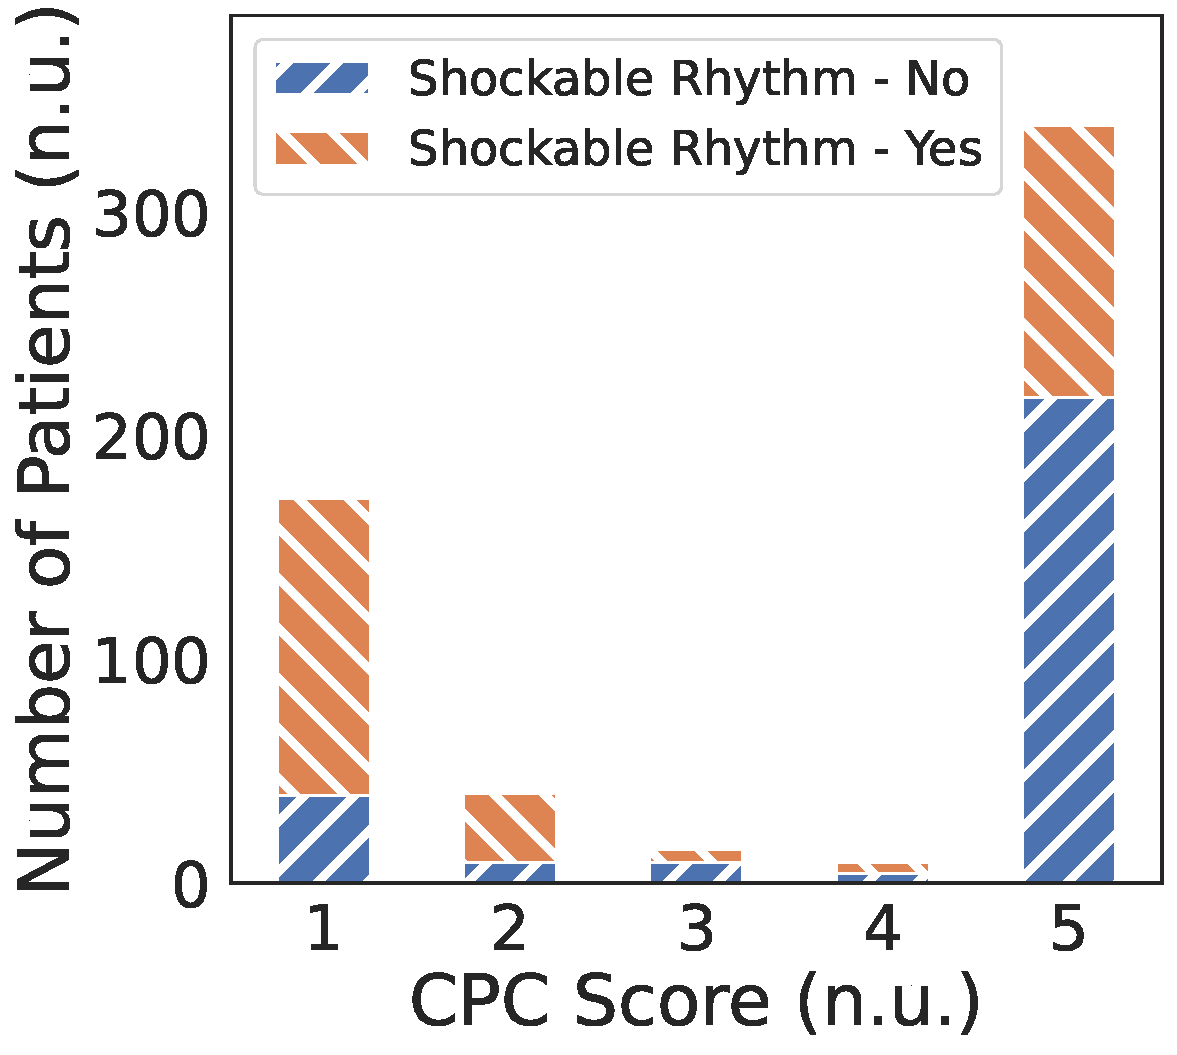
\includegraphics[width=\textwidth]{images/cpc-vfib-corr.pdf}
    \caption[]
    {Dist. against shockable rhythm.}
    \label{fig:cpc_vfib_corr}
\end{subfigure}
\hfill
\begin{subfigure}[t]{0.49\linewidth}
    \centering
    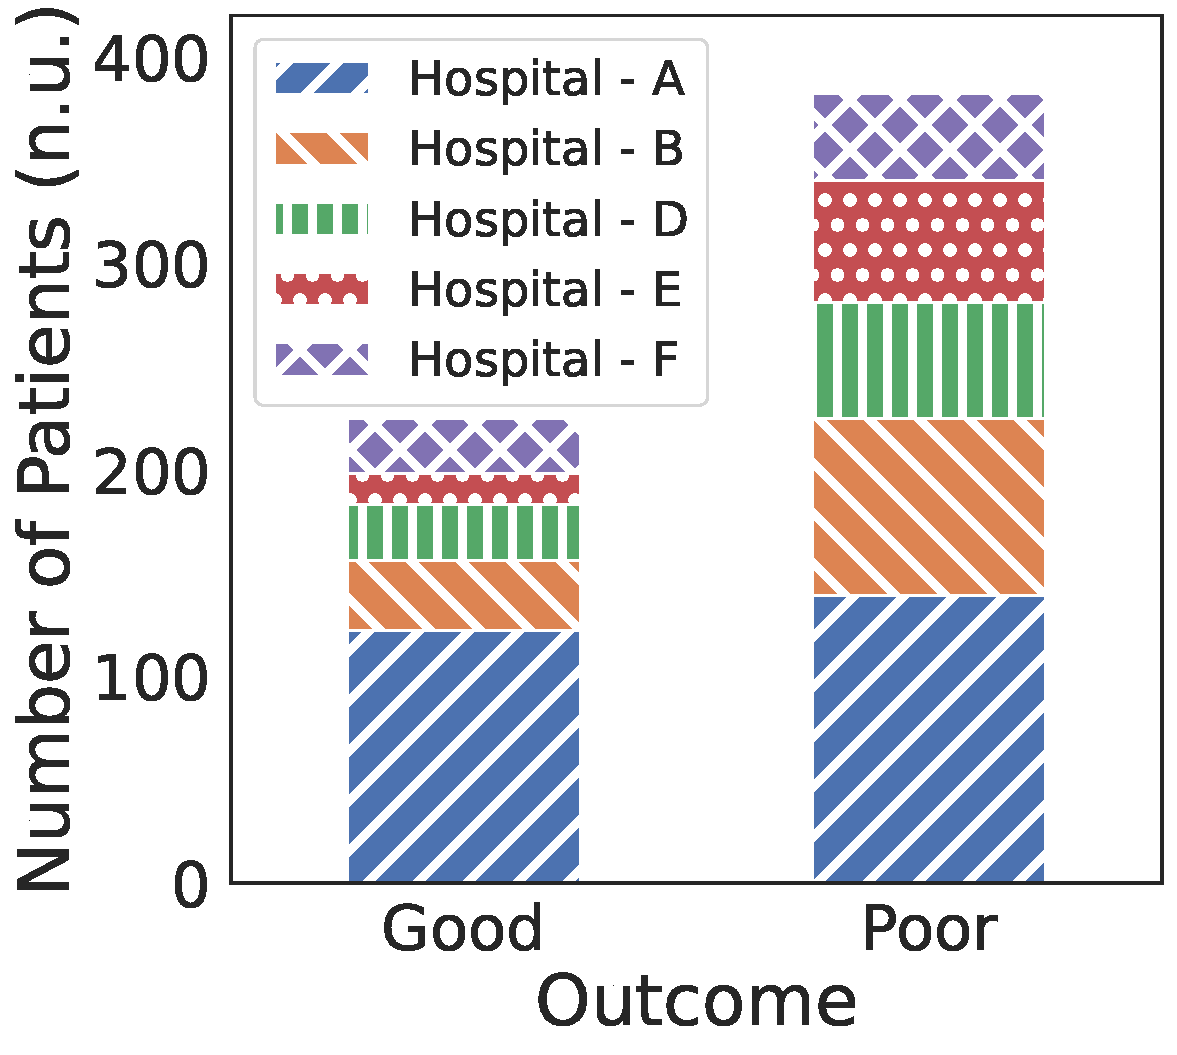
\includegraphics[width=\textwidth]{images/outcome-hospital-corr.pdf}
    \caption[]
    {Dist. against hospitals.}
    \label{fig:outcome_hospital_corr}
\end{subfigure}
\caption[]
{Distributions (Dist.) of the ``CPC Score'' and ``Outcome'' against 2 typical categorical metadata variables. Missing values for each variable were not counted.}
\label{fig:outcome_corr}
\end{figure}


The monitor for model selection is the Challenge score on a left-out validation set which was randomly selected and consisted of $20\%$ of the public training data. The Challenge score is defined as the largest TPR (true positive rate) such that FPR (false positive rate) $\le 0.05$ for the poor clinical outcome prediction. This agrees with the demand for methods with minimal false-positive rate of poor outcomes as introduced in Section \ref{sec:intro}.

A key tension for the Challenge objective lies in the existence of the large data and the limited computational resources (RAM and CPU time). As a consequence, further trade-offs were made: we randomly sliced a 3-minute (180 in the number of sample points) piece from each of the selected 5-minute epochs and loaded all the data pieces into memory every 5 training iterations. The rest primary training hyperparameters are collected in Table \ref{tab:hyperparams}. It should be noted that the maximum number of training iterations was set to 55 since almost all optimal models were obtained before 30 iterations in our offline experiments using much larger total iteration numbers (e.g. 100 iterations).

\begin{table}[!htp]
\centering
% requires packages boldline, multirow
\setlength\tabcolsep{2pt}
\begin{tabular}{@{\extracolsep{6pt}}c|c|c|c|c@{}}
\hlineB{3.5}
\multirow{2}{*}{batch size} & max & early stop & \multicolumn{2}{c}{learning rate} \\ \cline{4-5}
& \# iterations & patience & initial & max \\ \hline
32 & 55 & 25 & 2.5e-3 & 8e-3 \\
\hlineB{3.5}
\end{tabular}
\caption{Primary hyperparameters for NN model training. To avoid overfitting on the training data, early stop callbacks were set which were triggered if the best Challenge score on the left-out validation set stayed unchanged for 25 global iterations. The learning rates were set for the optimizer and its scheduler.}
\label{tab:hyperparams}
\end{table}



% \subsection{Minimum Guarantee Models}
% \label{subsec:min_grt_models}
% % almost finished

% The Challenge also evaluated the submissions on subsets with recordings truncated up to 12 / 24 / 48 hours from ROSC, in which case a single patient might not have valid EEGs. In order to be able to predict clinical outcomes without EEGs, we used a random forest model as a minimum guarantee model which took all clinical information of a patient provided by the I-CARE database as input. This model was selected via parameter grid searching over the same train-validation split as described in Section \ref{subsec:training}.


\section{Results}
\label{sec:results}

% almost finished

% The primary Challenge Score, which is the largest TPR such that FPR $\le 0.05$ evaluated on the hidden validation set up to 72 hours from ROSC, of our team ``Revenger'' was 0.701. Auxiliary scores evaluated on its truncated 12h / 24h / 48h subsets and scores on the training and cross-validation sets during the offline development of our solution are gathered in Table \ref{tab:challenge_scores}.

% % NOT finished
\begin{table}[!htp]
\centering
% requires packages boldline, multirow
\setlength\tabcolsep{2pt}
% \begin{tabular}{@{\extracolsep{6pt}}c|c|c|c|c@{}}
\begin{tabular}{c|c|c|c|c}
\hlineB{3.5}
& \multicolumn{4}{c}{\textbf{Challenge Scores}} \\ \cline{2-5}
& \textbf{72 hours} & 12 hours & 24 hours & 48 hours \\ \hline
Training & 0.814 $\pm$ 0.070 & - & - & - \\
Cross val. & 0.424 $\pm$ 0.026 & - & - & - \\ \hline
Hidden val. & \textbf{0.701} & 0.33 & 0.40 & 0.75 \\
Ranking & \textbf{5 / 270} & - & - & - \\
\hlineB{3.5}
\end{tabular}
\caption{Challenge score and ranking evaluated on the hidden validation set, scores on its truncated 12h / 24h / 48h subsets and scores on the training and cross-validation sets. Scores on the train and cross-validation sets are of the form $mean \pm std. dev.$ from all our offline experiments with z-score normalization included in the preprocessing pipeline.}
\label{tab:challenge_scores}
\end{table}


% It should be noted that the training and cross-validation data were de-identified, in which case different 180s data pieces were considered from different patients. This explains the lowered scores on these data subsets.

The primary Challenge Score, the largest TPR such that FPR $\le 0.05$ evaluated on the hidden test set up to 72 hours from ROSC, of our team ``Revenger'' was 0.554, ranked 12th out of 35 teams. This score and auxiliary scores from the truncated 48h / 24h / 12h subsets and the training and hidden validation sets are gathered in Table \ref{tab:final_results}.

% finished

\begin{table*}[t]
\centering

% requires packages boldline, multirow
% put the following in the preamble
% \usepackage{multirow}
% \usepackage{boldline}
% and probably one needs the following to make \textbf work
% \usepackage[T1]{fontenc}
\setlength\tabcolsep{6pt}
\setlength\extrarowheight{1pt}
\begin{tabular}{@{\extracolsep{4pt}}cclllllllll@{}}
\hlineB{3.5}
 &  &  & \multicolumn{2}{c}{\textbf{72h after ROSC}} & \multicolumn{2}{c}{48h after ROSC} & \multicolumn{2}{c}{24h after ROSC} & \multicolumn{2}{c}{12h after ROSC} \\
 &  &  & \textbf{Score} & \textbf{Rank} & Score & Rank & Score & Rank & Score & Rank \\
\hlineB{2.5}
\multicolumn{2}{c}{\multirow[c]{3}{*}{\textbf{Challenge Score}}} & \textbf{Test} & \textbf{0.554} & \textbf{12 / 35} & \textbf{0.54} & \textbf{13 / 35} & \textbf{0.257} & \textbf{28 / 35} & \textbf{0.252} & \textbf{15 / 35} \\
 &  & \textbf{Validation} & \textbf{0.701} & \textbf{3 / 35} & \textbf{0.746} & \textbf{1 / 35} & \textbf{0.403} & \textbf{16 / 35} & \textbf{0.328} & \textbf{12 / 35} \\
 &  & Training & 0.649 & 26 / 35 & 0.702 & 20 / 35 & 0.673 & 12 / 35 & 0.793 & 3 / 35 \\
\cline{1-11} \cline{2-11}
\multirow[c]{3}{*}{CPC} & \multirow[c]{3}{*}{MAE} & \textbf{Test} & \textbf{1.014} & \textbf{3 / 35} & \textbf{0.957} & \textbf{2 / 35} & \textbf{1.111} & \textbf{1 / 35} & \textbf{1.347} & \textbf{7 / 35} \\
 &  & \textbf{Validation} & \textbf{1.104} & \textbf{7 / 35} & \textbf{1.173} & \textbf{7 / 35} & \textbf{1.211} & \textbf{4 / 35} & \textbf{1.421} & \textbf{11 / 35} \\
 &  & Training & 0.871 & 19 / 35 & 0.844 & 13 / 35 & 0.888 & 9 / 35 & 0.806 & 3 / 35 \\
\cline{1-11} \cline{2-11}
\hlineB{3.5}
\end{tabular}
\caption{Challenge scores and rankings evaluated on the Training and the hidden Test/Validation sets, and on their truncated 48h / 24h / 12h subsets. MAE (mean absolute error) of CPC score predictions is also provided.}
\label{tab:final_results}
\end{table*}


 Despite the Challenge Score, our solution achieved remarkable results on MAE of CPC score predictions. We also include them in Table \ref{tab:final_results}.


\section{Discussion and Conclusions}
\label{sec:discu}

% almost finished.

As the results presented in Section \ref{sec:results} indicate, the TiCRNN model proposed in this work provides an effective solution to the problem of predicting the level of neurological recovery for comatose patients after cardiac arrest raised by the Challenge. It is relatively simple and lightweight, but still able to attain a TPR as high as 0.701 with FPR, which is vital for the patients in this problem, suppressed to a very low level ($\le 0.05$) for poor clinical outcome prediction. Another phenomenon that can be observed from Table \ref{tab:challenge_scores} is that the score on the hidden validation set is much higher than the score on the cross-validation set. This indicates that by combining results from multiple recordings, one is able to obtain a much more reliable prediction than from only one recording.

As introduced in Section \ref{subsec:data_selection} and \ref{subsec:training}, we made trade-offs for the limited computation resources by dropping a large proportion of the EEG data. The data amount (counting by time length) we really used for training the NN models merely constitutes 6 \% of the total EEG data. The potential of this extraordinarily big data had not yet been fully explored. Our team had planned to make full use of the data to train a larger model that learns latent representations from EEGs via unsupervised contrastive learning. However, due to the constraints of time and computation resources our team owns, we finally decided to stick to the TiCRNN model developed in the unofficial phase of the Challenge. Architecture design and unsupervised training mechanisms for large EEG models are left as future research directions.

The computation of SQI for EEGs as described in Section \ref{subsec:data_selection} is time-consuming. This prohibited us from adding a similar selection procedure in the pipeline of model evaluation on the hidden data and is highly probable to have a negative influence on our overall performance, especially for EEGs heavily contaminated with artifacts. Therefore, developing a faster and end-to-end SQI computation method would also be a meaningful research problem.

Despite the large EEG data amount, another nice feature of the I-CARE database is that it provides simultaneous electrocardiogram (ECG) signals along with the EEGs. This makes it possible to explore and develop multi-modal solutions to the Challenge problem, which is also a topic worth researching but not yet studied in this work.


%%%%%%%%%%%%%%%%%%%%%%%%%%%%%%%%%%%%%%%%%%%%%%%%%%%%%%%%%%%%%%%%%%%%%%%%%%%%%%%%

% acknowledgements

\section*{Acknowledgments}

% finished

The authors thank Professor Deren Han from Beihang University and Professor Wenjian Yu from BNRist, Tsinghua University for helping accomplish this work.


%%%%%%%%%%%%%%%%%%%%%%%%%%%%%%%%%%%%%%%%%%%%%%%%%%%%%%%%%%%%%%%%%%%%%%%%%%%%%%%%

\bibliographystyle{cinc}
\bibliography{references}

\begin{correspondence}
Jingsu Kang\\
No. 22, Qixiangtai Road, Heping District, Tianjin, China\\
kangjingsu@tmu.edu.cn,kjs890223@gmail.com
\end{correspondence}

\balance

\end{document}
